%!TEX root = main-cav.tex


%%%%%%%%%%%%%%%%%%%%%%%%%%%%%%%%%%%%%%%%%%%%%%%%
%%%%%%%%%%%%streaming numerical transducer%%%%%%%%%%%%%%%%
%%%%%%%%%%%%%%%%%%%%%%%%%%%%%%%%%%%%%%%%%%%%%%%%

\section{Streaming Numerical Transducers}\label{sec:def-snt}

In this section, we introduce \emph{streaming numerical transducers} (SNTs), whose inputs are data words and outputs are integer values. A SNT scans a data word from left to right, records and aggregates information using control and data variables, and outputs an integer value when it finishes reading the data word. We will use SNTs to decide the commutativity and equivalence problem of the reducer programs defined in Section~\ref{sec-mr-prog}. 
Due to lack of space we omit most of the proofs in the conference version. The complete paper is available at~\cite{full-version}. 


A SNT $\Ss$ is a tuple $(Q, X, Y, \delta, q_0, O)$ where $Q$ is a finite set of states, $X$ is a finite set of control variables to store data values that have been met, $Y$ is a finite set of data variables to aggregate information for the output, $\delta$ is the set of transitions, $q_0 \in Q$ is the initial state, $O$ is the output function, which is a partial function from $Q$ to $\Ee_{X \cup Y}$.%\zhilin{Here the variable $\cur$ should not be used.}
The set of transitions $\delta$ comprises the tuples $(q,  g, \eta, q')$, where $q,q'\in Q$, $g$ is a guard over $X^+$ (defined in Section~\ref{sec:preliminaries}), and $\eta$ is an assignment which is a partial function mapping $X \cup Y$  to $\Ee_{X^+ \cup Y}$ such that for each $x \in \dom(\eta) \cap X$, $\eta(x)=x'$ for some $x' \in X^+$. We write $q \xrightarrow{(g,\eta)} q'$ to denote $(q,g,\eta,q') \in \delta$ for convenience.  We would like to remark that the guards in the transitions can be of both types, that is, of type 1 or type 2.

Moreover, we assume that an SNT $\Ss$ satisfies the following constraints. (1) \emph{Deterministic:} For each pair of distinct transitions originating from $q$, say $(q, g_1, \eta_1,q'_1)$ and $(q, g_2,\eta_2,q'_2)$, it holds that $g_1 \wedge g_2$ is unsatisfiable. (2) \emph{Generalized flat:} Each SCC (strongly connected component) of the transition graph of $\Ss$ is either a single state or a set of simple cycles $\{C_1,\dots, C_n\}$ which contains a state $q$ such that for each $i,j: 1 \le i < j \le n$, $q$ is the \emph{only} state shared by $C_i$ and $C_j$. (3) \emph{Independently evolving and copyless:} For each $(q, g, \eta, q') \in \delta$ and for each $y \in \dom(\eta) \cap Y$, $\eta(y)=e$ or $\eta(y)=y+e$ for some expression $e$ over $X^+$.

The semantics of an SNT $\Ss$  is defined as follows. A \emph{configuration} of $\Ss$ is a pair $(q,\rho)$, where $q \in Q$ and $\rho$ is a valuation of $X \cup Y$. An \emph{initial} configuration of $\Ss$ is $(q_0,\rho_0)$, where $\rho_0$ assigns arbitrary values to the variables from $X\cup Y$.
A sequence of configurations $(q_0,\rho_0)(q_1,\rho_1)\ldots(q_n,\rho_n)$ is
a \emph{run} of $\Ss$ over a data word $w=d_1 \dots d_n$ iff there exists a path (sequence of transitions) $P=q_0 \xrightarrow{(g_1,\eta_1)} q_1 \xrightarrow{(g_2,\eta_2)} q_2 \dots q_{n-1} \xrightarrow{(g_n, \eta_n)} q_n$ such that for each $i \in [n]$, $\rho_{i-1}[d_i/\cur] \models g_i$, and $\rho_i$ is obtained from $\rho_{i-1}$ as follows: (1) For each $x \in X$, if $\eta_i(x)=\cur$, then $\rho_i(x)=d_i$, otherwise, if $\eta_i(x)=x' \in X$, then $\rho_i(x)=\rho_{i-1}(x')$. (2) For each $y \in Y$, if $y \in \dom(\eta_i)$, then $\rho_i(y)=\eval{\eta_i(y)}{\rho_{i-1}[d_i/\cur]}$, otherwise, $\rho_i(y)=\rho_{i-1}(y)$.
We call $(q_n,\rho_n)$ the \emph{final configuration} of the run. In this case, we also say that the run follows the path $P$.
We say that a path $P$ in $\Ss$ is \emph{feasible} iff there exists a run of $\Ss$ following $P$. 
An SNT $\Ss$ is said to be \emph{transition-enabled} if each path in $\Ss$ is feasible. We assume that all SNTs considered in this paper are transition enabled.
%We say that $(q_i,\rho_i)$ is \emph{reachable} from $(q_0,\rho_0)$, for $i \in [n]$.

%We would like to remark that since $\Ss$ is deterministic, for each data word $w$, if there is a run of $\Ss$ over $w$, then there is exactly one path $P$ of $\Ss$ (recall the aforementioned transition-enabled assumption) such that for each initial configuration $(q_0,\rho_0)$, the  run of $\Ss$ over $w$ starting from $(q_0,\rho_0)$ follows $P$. 

Given a data word $w = d_1 \dots d_n$ and an initial configuration $(q_0, \rho_0)$, if there is a run of $\Ss$ over $w$ starting from $(q_0,\rho_0)$ and with the final configuration $(q_n,\rho_n)$, then the output of $\Ss$ over $w$ w.r.t. $\rho_0$, denoted by ${\Ss}_{\rho_0}(w)$, is $\eval{O(q_n)}{\rho_n}$. Otherwise, ${\Ss}_{\rho_0}(w)$ is undefined, denoted by $\bot$. 


\begin{example}[SNT for max]
The SNT $\Ss_{\max}$ for computing the maximum value of an input data word is defined as $(\{q_0,q_1\}, \{\maxv\}, \emptyset, \delta, q_0, O)$, where the set of transitions $\delta$ and the output function $O$ are illustrated in Fig.\ref{fig-snt-exmp}
%such that $\delta = \{(q_0, \ltrue, \maxv:=\cur, q_1), (q_1, \maxv < \cur, \maxv:=\cur,q_1), (q_1, \maxv \ge \cur, \emptyset, q_1)\}$ and $O(q_1)=\maxv$, 
%
(here $X=\{\maxv\}$, $Y=\emptyset$, and $\maxv:=\cur$ denotes the assignment of $\cur$ to the variable $\maxv$).
\begin{figure}[htbp]
\begin{center}
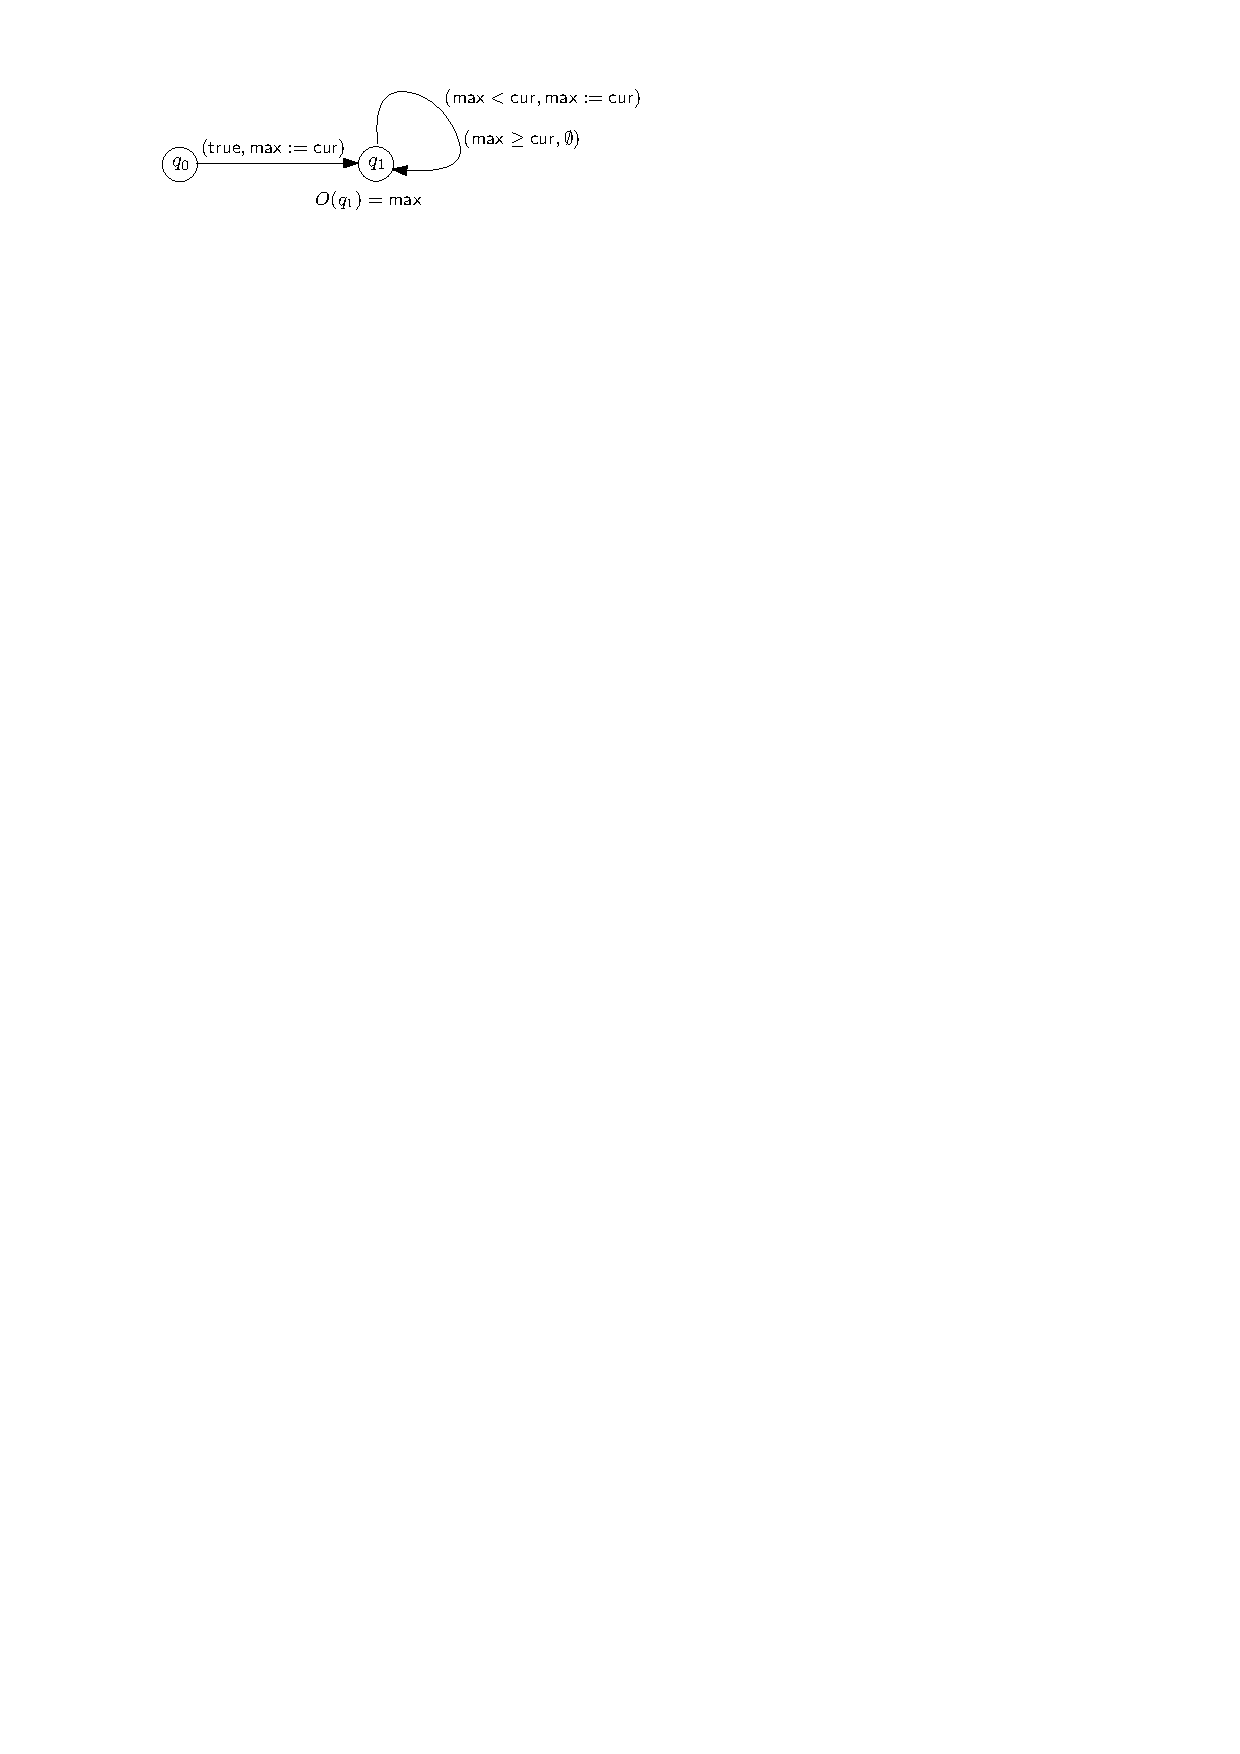
\includegraphics{snt-exmp.pdf}
\caption{The SNT $\Ss_{\max}$ for computing the maximum value}
\label{fig-snt-exmp}
\end{center}
\end{figure}
\end{example}

\vspace{-12mm}


%\begin{example}[SNT for sum]
%$\Ss_{\mathrm{sum}}=(\{q_0,q_1\}, \emptyset, \{\sumv\}, \delta, q_0, O)$ such that %$\delta=\{(q_0, \ltrue, \sumv:=\cur, q_1), (q_1, \ltrue, \sumv:=\sumv + \cur, q_1)$, and %$O(q_1)=\sumv$. 
%\end{example
\begin{proposition}\label{prop-mrprog-to-snt}
For each reducer program $p$, one can construct an equivalent SNT $\Ss$ where the number of states and the maximum number of simple cycles in an SCC of the transition graph are at most exponential w.r.t. the number of branching statements in $p$. 
\end{proposition}
%We describe the procedure translating a program $p$ into an SNT $\Ss$ in the appendix. 
Intuitively, the exponential blow-up in the construction is due to the following difference between reducer programs $p$ and SNTs $\Ss$: A reducer program moves to the next value of an input data word only when a $\nnext$ statement is executed, while an SNT advances the iterator in each transition. Therefore, a sequence of statements with $k$ branching points between each pair of consecutive $\nnext$ statements in the control flow of $p$ correspond to at most $2^k$ transitions of $\Ss$.



%We first compute a fixed point $\defval$ inductively as follows. 
%\begin{enumerate}
%\item Initially, let $\defval_0=\{(q_0,\emptyset)\}$.
%
%\item For each $i > 0$, compute $\defval_i$ from $\defval_{i-1}$ as follows,
%\begin{itemize}
%\item each element of $\defval_{i-1}$ is an element of $\defval_i$, 
%
%\item for each $(q,Z) \in \defval_{i-1}$ and each transition $(q,g,\eta,q') \in \delta$,  let $Z' = Z \cup (X \cap \dom(\eta)) \cup \{y \in Y \cap \dom(\eta) \mid \vars(\eta(y)) \subseteq Z \cup \{\cur\}\}$, put $(q',Z')$ into $\defval_i$.
%\end{itemize}
%
%\item If $\defval_{i-1}=\defval_i$, then the computation stops, otherwise, let $i:=i+1$ and the computation continues.
%\end{enumerate}

We focus on three decision problems of SNTs: (1) \emph{Commutativity}: Given an SNT $\Ss$, decide whether $\Ss$ is commutative, that is, whether for each data word $w$ and each permutation $w'$ of $w$, $\Ss_{\rho_0}(w)=\Ss_{\rho_0}(w')$ for all initial valuations $\rho_0$. (2) \emph{Equivalence}: Given two SNTs $\Ss,\Ss'$, decide whether $\Ss$ and $\Ss'$ are equivalent, that is, whether over each data word $w$, $\Ss_{\rho_0}(w)=\Ss'_{\rho_0}(w)$ for all initial valuations $\rho_0$. (3) \emph{Non-zero output}: Given an SNT $\Ss$, decide whether $\Ss$ has a non-zero output, that is, whether there is a data word $w$ and initial valuations $\rho_0$ such that $\Ss_{\rho_0}(w)\notin \{\bot, 0\}$. 

We first observe that the commutativity problem can be reduced to the equivalence problem of SNTs, which can be further reduced to the non-zero output problem of SNTs. For analyzing the complexity of the decision procedure in the next section,  we state the complexity of the reductions w.r.t. the following factors of SNTs: the number of states, the number of control variables (resp. data variables), and the maximum number of simple cycles in an SCC of the transition graph. We will adopt the convention that if after a reduction, some factor becomes exponential, then this fact will be stated explicitly, and on the other hand, if some factor is still polynomial after the reduction, then this fact will be made implicit and will not be stated explicitly. 

\vspace{-1mm}
\begin{proposition}\label{prop-snt-cmm-to-eqv}
The commutativity problem of SNTs is reduced to the equivalence problem of SNTs in polynomial time.
%, where the number of states of SNTs obtained after the reduction is at most exponential over the number of control variables. 
\end{proposition}

We briefly describe the idea of the reduction in Proposition~\ref{prop-snt-cmm-to-eqv} here. Suppose that $\Ss=(Q, X, Y, \delta, q_0, O)$ is an SNT such that $X=\{x_1,\dots,x_k\}$ and $Y=\{y_1,\dots,y_l\}$. Without loss of generality, we assume that the output of $\Ss$ is defined only for data words of length at least two. We will construct two SNTs $\Ss_1$ and $\Ss_2$ so that $\Ss$ is commutative iff $\Ss$ is equivalent to both $\Ss_1$ and $\Ss_2$.
\begin{itemize}
\item Intuitively, over a data word $w=d_1 d_2 d_3 \dots d_n$ with $n\ge 2$, $\Ss_1$ simulates the run of $\Ss$ over $d_2 d_1 d_3 \dots d_n$, that is, the data word obtained from $w$ by swapping the first two data values.
%
\item Intuitively, over a data word $w=d_1 d_2 d_3 \dots d_n$ with $n\ge 2$, $\Ss_2$ simulates the run of $\Ss$ over $d_2 d_3 \dots d_n d_1$, that is, the data word obtained from $w$ by moving the first data value to the end. 
\end{itemize}
The correctness of this reduction follows from the fact that all the permutations of $d_1\dots d_n$ can be generated by composing the two aforementioned permutations corresponding to $\Ss_1$ and $\Ss_2$ respectively (cf. Proposition 1 in \cite{CHSW15}). The construction of $\Ss_1$ (resp. $\Ss_2$) from $\Ss$ is in  polynomial time w.r.t. the size of $\Ss$.
%, while the construction of $\Ss_2$ from $\Ss$ involves an exponential blow-up w.r.t. the number of control variables, which is attributed to the determinism of SNTs.

\begin{proposition}\label{prop-snt-eqv-to-nzero}
From SNTs $\Ss_1$ and $\Ss_2$, an SNT $\Ss_3$ can be constructed in polynomial time such that  $(\Ss_1)_{\rho_0}(w) \neq (\Ss_2)_{\rho_0}(w)$ for some  data word $w$ and valuation $\rho_0$  iff $(\Ss_3)_{\rho_0}(w) \not\in \{\bot,0\}$ for some data word $w$ and valuation $\rho_0$. 
\end{proposition}
Proposition~\ref{prop-snt-eqv-to-nzero} can be proved by a straightforward product construction.

The lemma below states a property of SNTs, due to the fact that the guards are equality-free (cf. the definition of guards in Section~\ref{sec:preliminaries}) and SNTs are transition-enabled.

\begin{proposition}\label{prop-snt-distinct-value}
Let $\Ss$ be an SNT and $P$ be a path in $\Ss$. There is a data word $w$ such that (1) there is a run of $\Ss$ over $w$ which follows $P$, (2) no data values occur twice in~$w$.
\end{proposition}



%%%%%%%%%%%%%%%%%%%%%%%%%%%%%%%%%%%%%%%%%%%%%%
%%%%%%%%%%%%%%%%%%%%%%%%%%%%%%%%%%%%%%%%%%%%%%
\hide{
\smallskip

\noindent {\it Reachability graph}.
Given an SNT  $\Ss=(Q, X, Y, \delta, q_0, O)$, we define the \emph{reachability graph} to help deciding if a path in $\Ss$ is feasible.  Let $c_{min}$ and $c_{max}$ denote the minimum resp. maximum integer constant occurring in the guards of the transitions in $\delta$. If no integer constant occurs in the guards, then $c_{min}=c_{max}=0$. Let $\sntcset$ be the set of all total preorders $\preceq$ over $X\cup[c_{min},c_{max}]$ such that $\preceq$ enforces the natural order between the constants in $[c_{min},c_{max}]$.  We use $\sim_{\preceq}$ to denote the equivalence relation induced by $\preceq$.
Formally, a reachability graph $G_\Ss=(n_0,N, E)$ consists of the set of nodes $N \subseteq Q\times \sntcset$, the set of labeled arcs $E \subseteq N\times \delta\times N$, and the initial node $n_0=(q_0, \preceq_0)$, where $\preceq_0 \in \sntcset$ is the preorder that forces all variables in $X$ equivalent to zero. We write $n \xrightarrow{t} n'$ to denote $(n,t,n') \in E$.
For $q \in Q$, we use $N_q$ to denote the set of nodes in $N$ corresponds to $q$, i.e., the set $\{(q, \preceq) \in N \mid \preceq \in \sntcset \}$.

Our intention is that $G_\Ss$ encodes the reachability relation between configurations of $\Ss$. For this, we need relate the runs of $\Ss$ with the paths in $G_\Ss$, which is formally defined here. A configuration $\rho$ of $\Ss$ \emph{conforms to} $\preceq \in \sntcset$ if for each $x,x' \in X$ (resp. $x \in X$ and $c \in [c_{min}, c_{max}]$), $\rho(x) \le \rho(y)$ iff $x \preceq x'$ (resp. $\rho(x) \le c$ iff $x \preceq c$ and $c \le \rho(x)$ iff $c \preceq x$).   A run $(q_0,\rho_0)(q_1,\rho_1)\ldots(q_n,\rho_n)$ corresponding to  a path $P= t_1 t_2 \ldots t_n$ in $\Ss$ is said to \emph{conform to}  a path in $G_\Ss$ if the path is of the form $(q_0, \preceq_0) \xrightarrow{t_1} (q_1, \preceq_1) \xrightarrow{t_2} \ldots \xrightarrow{t_n} (q_n, \preceq_n)$, and for each $j \in [0,n]$, $\rho_j$ conforms to $\preceq_j$.

\begin{proposition}\label{prop-snt-norm}
	From each SNT $\Ss=(Q, X, Y, \delta, q_0, O)$, one can construct a  reachability graph $G_\Ss=(n_0,N, E)$ with the following property: Each run of $\Ss$ conforms to some path in $G_\Ss$, and each path of $G_\Ss$ has a run of $\Ss$ conforming to it.  
%for any path $n_0 \xrightarrow{t_0} n_1 \xrightarrow{t_1} \ldots n_{m-1} \xrightarrow{t_{m-1}} n_m $ in $G_\Ss$, (1) $P=t_0t_1\ldots t_{m-1}$ is feasible in $\Ss$, and (2) let $n_m=(q,f)$, then for each run corresponding to P, the final configuration of the run conforms to $f$.
Moreover, the size of $N$ is at most exponential in the size of $X$. 
\end{proposition}
}

%
%The idea of the construction is simple. 
%To ensure the constructed SNT is well-defined, we record in the states the set of variables whose values are defined, and change the transitions and the output function accordingly.
%To ensure the ``uniquely-valued'' constraint, we add the constraint $\bigwedge_{x \in X} \cur \neq x$ into the guard when $\cur$ is stored into some control variable. 
%To ensure the ``transition-enabled'' constraint and ``state dominating'' constraint, we record in the states the equivalence relation and order relation between the control variables, as well as their relation with the constants from $[c_{min}, c_{max}]$, and enforce that the guards in the transitions conform to these relations recorded in the states, which guarantees that all the transitions are enabled.

\hide{
\yfc{Old version:}
An SNT $\Ss=(Q,X,Y,\delta,q_0,O)$ is said to be \emph{normalized} if the following constraints are satisfied:
(1) \emph{Well-defined}: For each run $(q_0,\rho_0) \dots (q_n,\rho_n)$ of $\Ss$ corresponding to the path $q_0 \xrightarrow{(g_1,\eta_1)} q_1 \dots q_{n-1} \xrightarrow{(g_n,\eta_n)} q_n$, and each $i \in [n]$, it holds that $\rho_{i}(z) \neq \bot$ for all $z \in \dom(\eta_i)$, 
%more formally, it holds that $\vars(\eta_i(z)) \subseteq \{z' \mid \rho_i(z') \neq \bot\} \cup \{\cur\}$, 
%
moreover, if $O(q_n)$ is defined, then $\rho_n(z)\neq\bot$ for all  $z\in \vars(O(q_n))$. (2) \emph{Uniquely-valued}: For each $(q,g,\eta,q') \in \delta$, if $\eta(x)=\cur$ for some $x \in X$, then the guard $g$ implies $\bigwedge_{x \in X} \cur \neq x$.  Intuitively, when the current data value $\cur$ is stored into some control variable, it is required that $\cur$ is distinct from all the data values that have already been stored in the control variables. (3) \emph{Transition-enabled}: Every sequence of transitions $q_0 \xrightarrow{(g_1,\eta_1)} q_1 \dots q_{n-1} \xrightarrow{(g_n,\eta_n)} q_n$ in $\Ss$ has at least one corresponding run. (4) \emph{State-dominating}: For each state $q \in Q$, and every pair of valuations $\rho,\rho'$ such that $(q,\rho)$ and $(q,\rho')$ are reachable from the initial configuration $(q_0,\rho_0)$, it holds that $\rho,\rho'$ are equivalent in the following sense: For each guard $g \in \{x_i < x_j \mid 1 \le i, j \le k\} \cup \{x_i = c \mid 1 \le i \le k, c_{min} \le c \le c_{max} \} \cup \{x_i < c_{min},x_i > c_{max}  \mid 1 \le i \le k\}$, $\rho \models g$ iff $\rho' \models g$.


%\yfc{New version:}
An SNT $\Ss=(Q,X,Y,\delta,q_0,O)$ is said to be \emph{normalized} if the following constraints are satisfied:
(1) \emph{Transition-enabled}: Every sequence of transitions $q_0 \xrightarrow{(g_1,\eta_1)} q_1 \dots q_{n-1} \xrightarrow{(g_n,\eta_n)} q_n$ in $\Ss$ has at least one corresponding run. (2) \emph{State-dominating}: For each state $q \in Q$, and every pair of valuations $\rho,\rho'$ such that $(q,\rho)$ and $(q,\rho')$ are reachable from the initial configuration $(q_0,\rho_0)$, it holds that $\rho,\rho'$ are equivalent in the following sense: For each guard $g \in \{x_i < x_j \mid 1 \le i, j \le k\} \cup \{x_i = c \mid 1 \le i \le k, c_{min} \le c \le c_{max} \} \cup \{x_i < c_{min},x_i > c_{max}  \mid 1 \le i \le k\}$, $\rho \models g$ iff $\rho' \models g$.

% $(q, g, \eta, q') \in \delta$, the guard $g$ implies one of the followings: $\cur < c_{min}$, $\cur = c$ for $c_{min} \le c \le c_{max}$, or $\cur > c_{max}$. 
%
%(3) \emph{Constant-partitioned}: For each $(q, g, \eta, q') \in \delta$, the guard $g$ implies one of the followings: $\cur < c_{min}$, $\cur = c$ for $c_{min} \le c \le c_{max}$, or $\cur > c_{max}$. 
\begin{proposition}\label{prop-snt-norm}
	From each SNT, one can construct an equivalent normalized SNT whose number of states is at most exponential w.r.t. the number of control variables. 
\end{proposition}
%
The idea of the construction is simple. 
%To ensure the constructed SNT is well-defined, we record in the states the set of variables whose values are defined, and change the transitions and the output function accordingly.
%To ensure the ``uniquely-valued'' constraint, we add the constraint $\bigwedge_{x \in X} \cur \neq x$ into the guard when $\cur$ is stored into some control variable. 
To ensure the ``transition-enabled'' constraint and ``state dominating'' constraint, we record in the states the equivalence relation and order relation between the control variables, as well as their relation with the constants from $[c_{min}, c_{max}]$, and enforce that the guards in the transitions conform to these relations recorded in the states, which guarantees that all the transitions are enabled.

}